\chapter{Appendix}
\label{chap:appendix}

\section{Data set}
\label{sec:data_set}
WiFi traces were taken over the	course of several weeks in an office space.
The office space has seven work places (not all of them being regularly occupied), which are placed in partially separated compartments, and a fully sound insulated meeting chamber.
The devices associated with the AP are typically the laptops of the people working in the office plus, sometimes, their mobile phones. Additionally there are a few desk-top computers that are being used for data collection and storage.

Figure \ref{fig:day299} visualises the total amount of traffic over time that is being sent by the WiFi AP to various associated clients
  during one afternoon in the office, along with packet airtimes (inversely proportional to the transmission rates) 
  with which individual packets are being transmitted.
  Each panel shows the number of data frames being transmitted to one particular client as a function of time.
  The full red histograms are the logarithm ({\sf log$_{10}$}) of the number of acknowledged frames per five-minute time bin,
  the open (inverted) histograms are the number of Non-acknowledged frames. The blue dots are the logarithm ({\sf log$_{10}$}) of the
  “airtime” being used at a given point in time. The airtime is the one listed in the trace header
  (i.e., the airtime  assumed by Minstrel for a typical data packet).


 \begin{figure}
      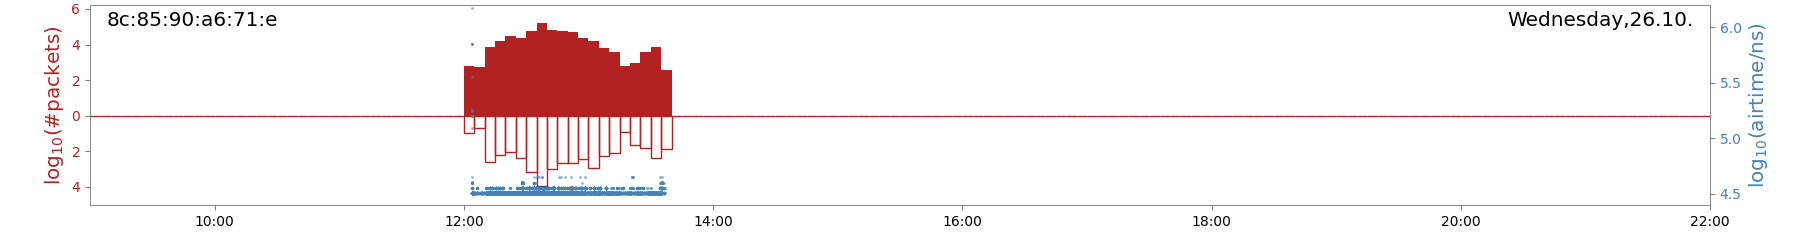
\includegraphics[width=\textwidth]{figures/Appendix/a.png}
      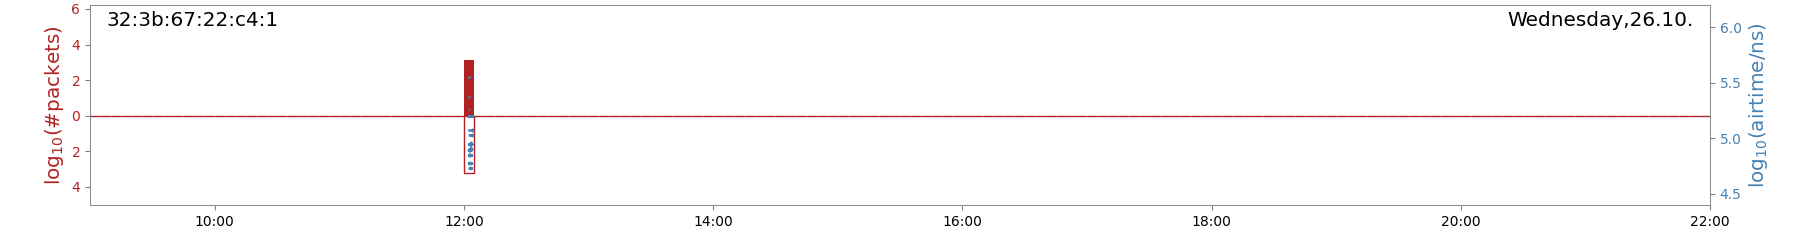
\includegraphics[width=\textwidth]{figures/Appendix/d299_32:3b:67:22:c4:1_pkts_shft.png}
      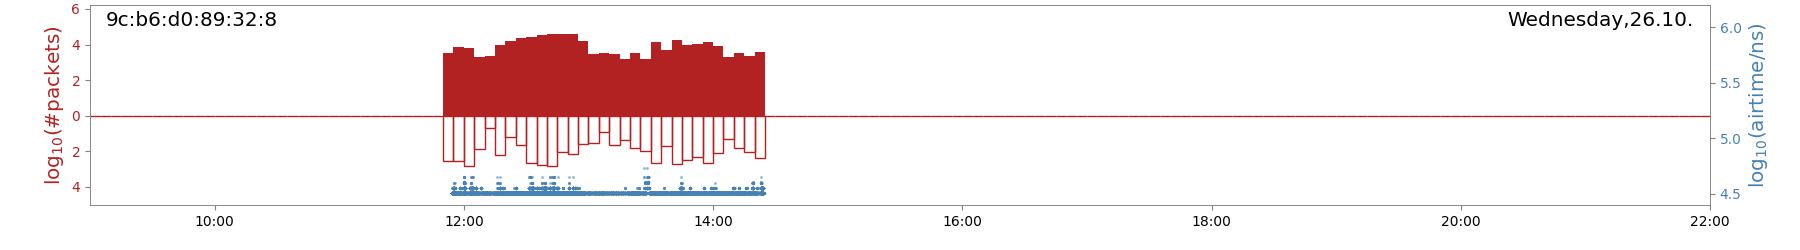
\includegraphics[width=\textwidth]{figures/Appendix/d299_9c:b6:d0:89:32:8_pkts_shft.png}
      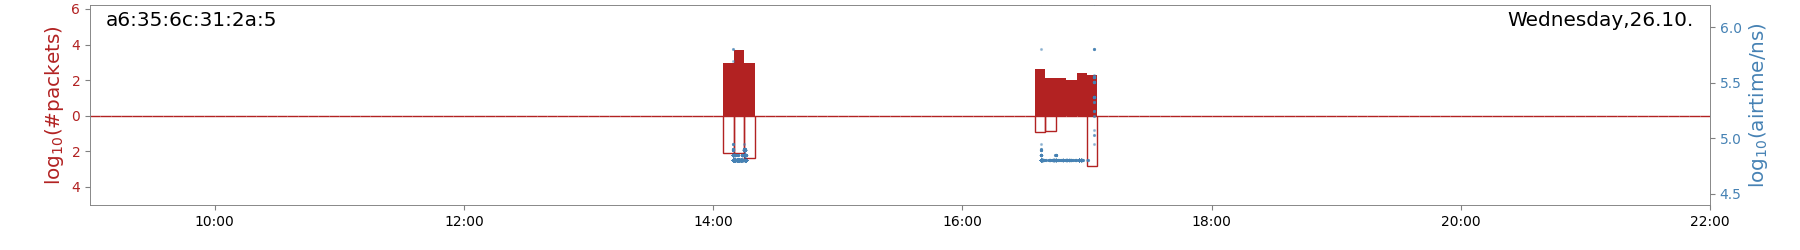
\includegraphics[width=\textwidth]{figures/Appendix/d299_a6:35:6c:31:2a:5_pkts_shft.png}
      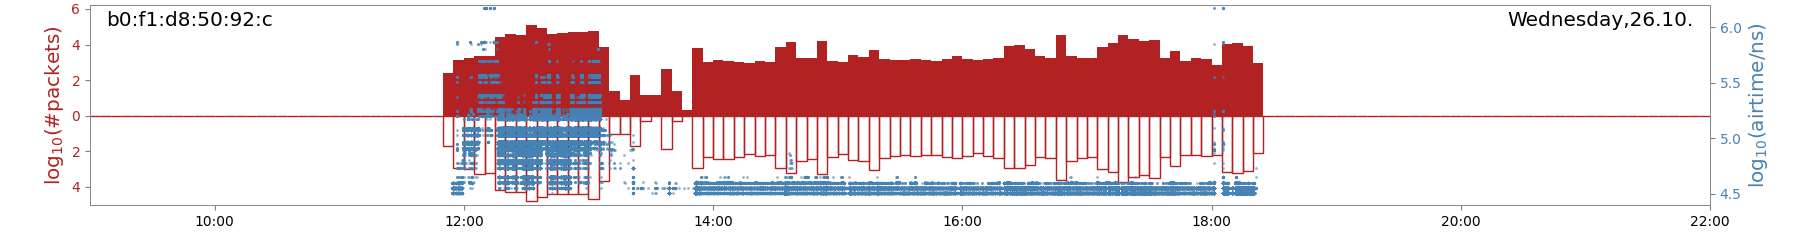
\includegraphics[width=\textwidth]{figures/Appendix/d299_b0:f1:d8:50:92:c_pkts_shft.png}
      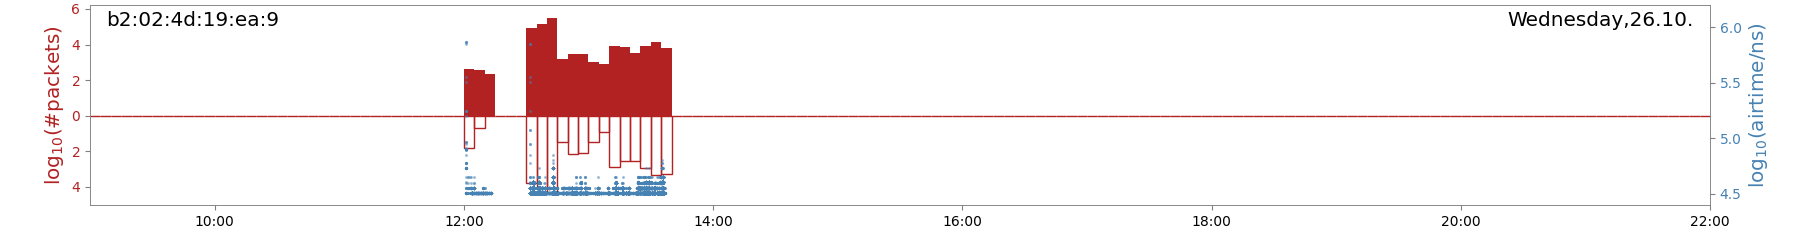
\includegraphics[width=\textwidth]{figures/Appendix/d299_b2:02:4d:19:ea:9_pkts_shft.png}
      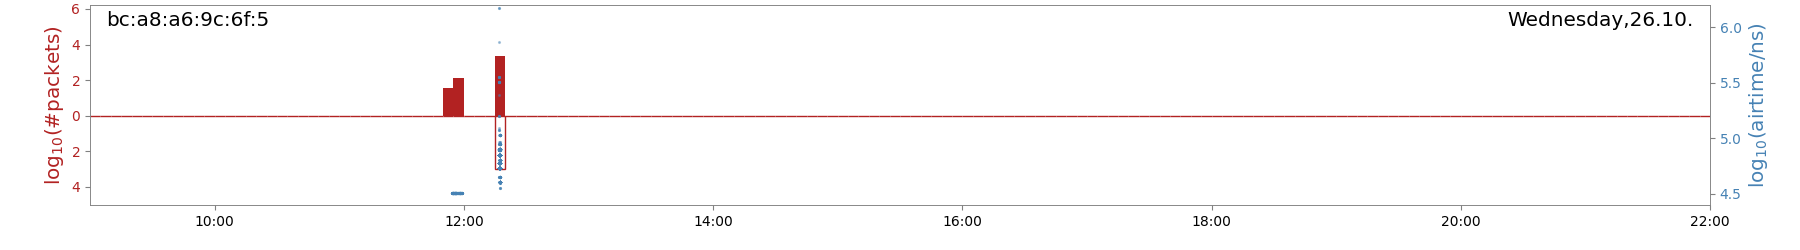
\includegraphics[width=\textwidth]{figures/Appendix/d299_bc:a8:a6:9c:6f:5_pkts_shft.png}
      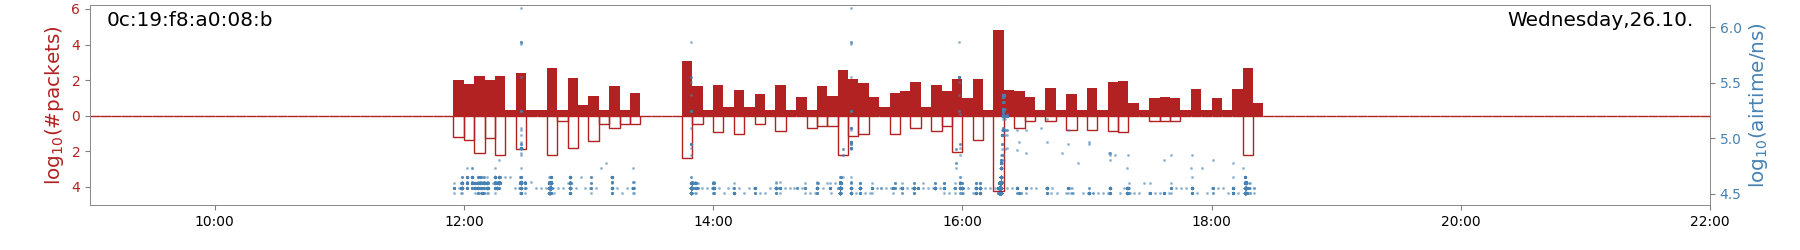
\includegraphics[width=\textwidth]{figures/Appendix/d299-0c:19:f8:a0:08:b-pkts-shft.png}
      \caption[WiFi Traffic]{WiFi traffic and airtimes (inversely proportional to the transmission rates) for associated clients on October 26th, 2022.
      Taken from~\cite{SNCX_internal_note}}
      \label{fig:day299}
 \end{figure}


% \begin{figure}
%   \centering
%   \includegraphics[width=0.9\textwidth]{figures/Appendix/d299_0c:19:f8:a0:08:b_pkts_shft.png}
%   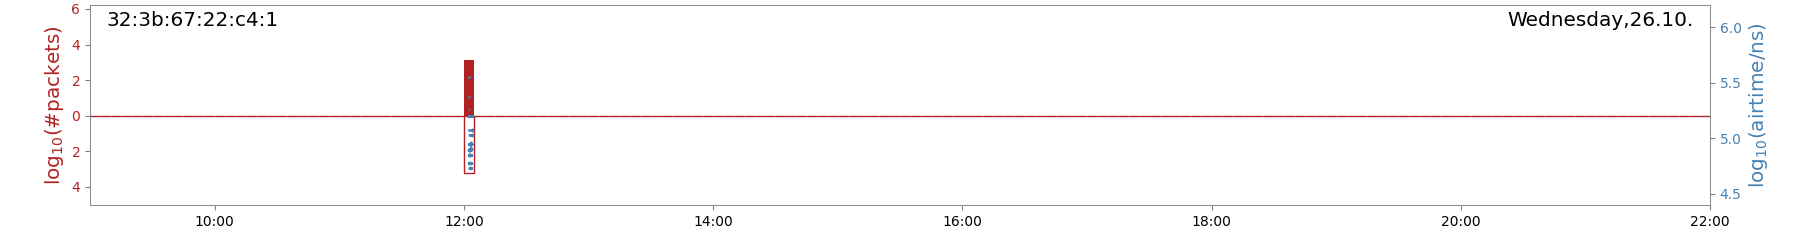
\includegraphics[width=0.9\textwidth]{figures/Appendix/d299_32:3b:67:22:c4:1_pkts_shft.png}
%   \includegraphics[width=0.9\textwidth]{figures/Appendix/d299_8c:85:90:a6:71:e_pkts_shft.png}
%   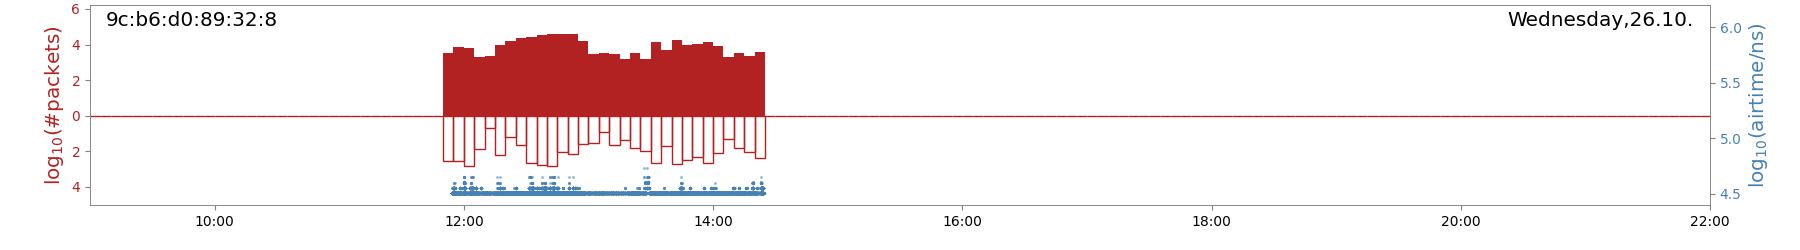
\includegraphics[width=0.9\textwidth]{figures/Appendix/d299_9c:b6:d0:89:32:8_pkts_shft.png}
%   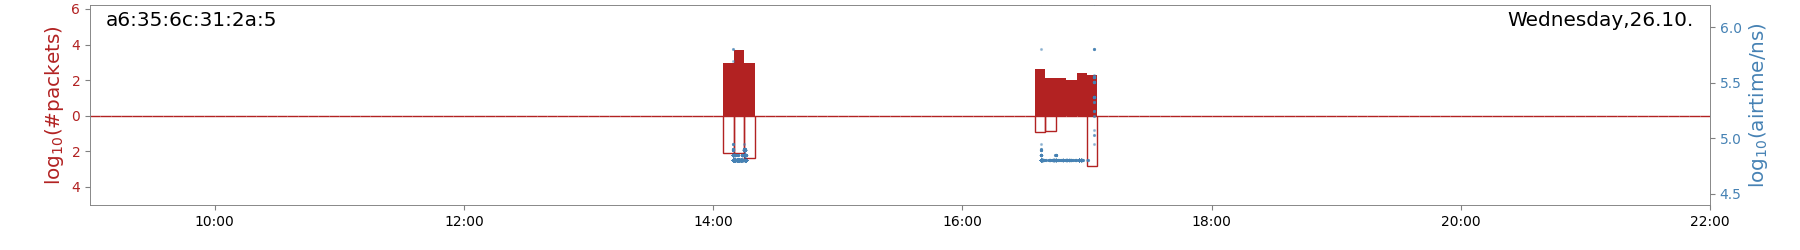
\includegraphics[width=0.9\textwidth]{figures/Appendix/d299_a6:35:6c:31:2a:5_pkts_shft.png}
%   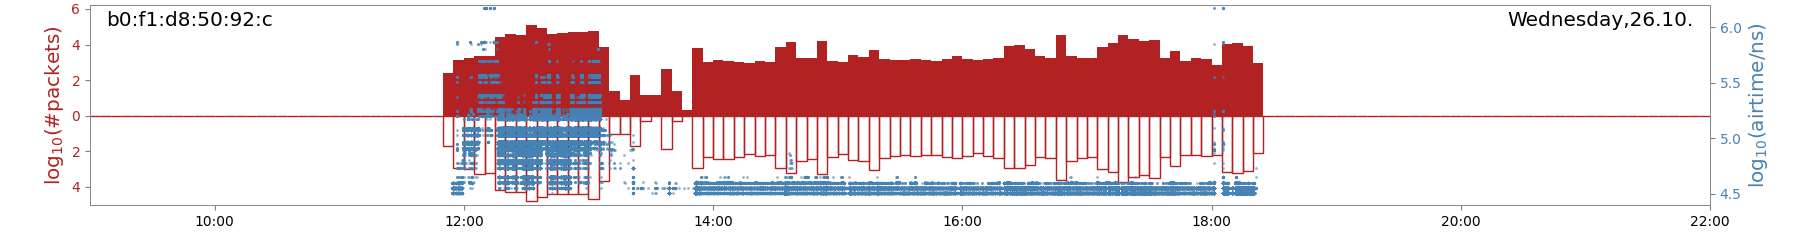
\includegraphics[width=0.9\textwidth]{figures/Appendix/d299_b0:f1:d8:50:92:c_pkts_shft.png}
%   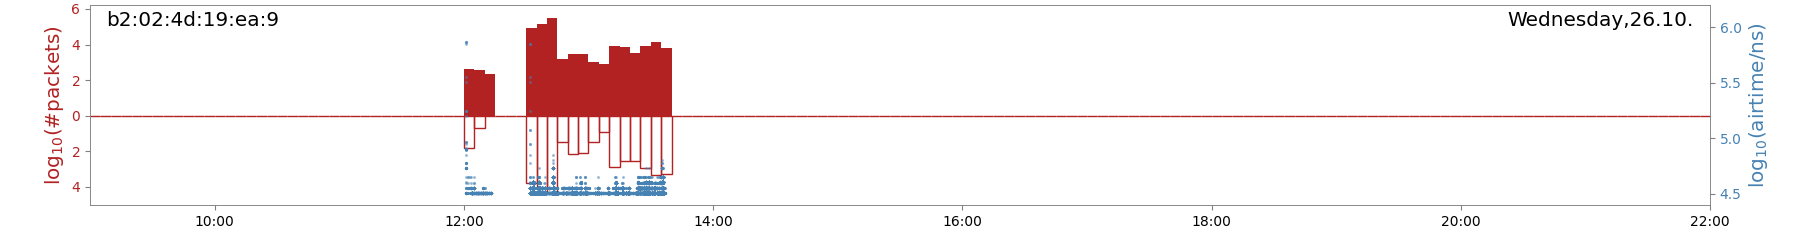
\includegraphics[width=0.9\textwidth]{figures/Appendix/d299_b2:02:4d:19:ea:9_pkts_shft.png}
%   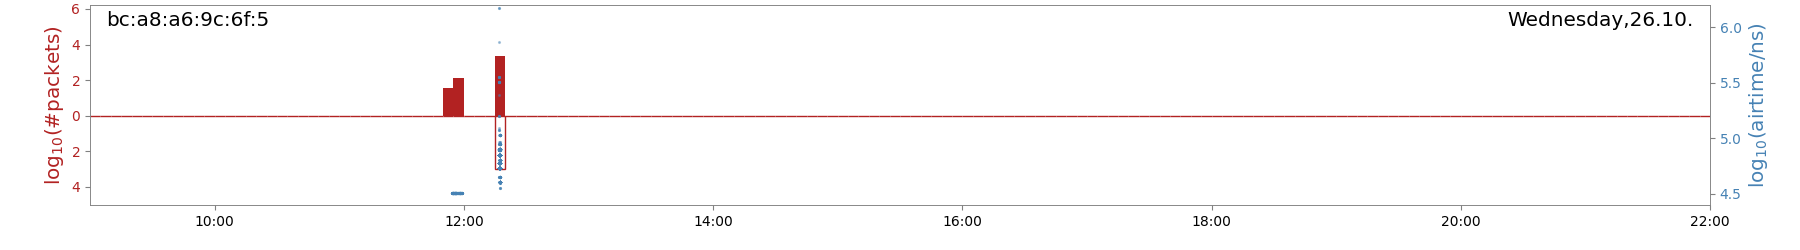
\includegraphics[width=0.9\textwidth]{figures/Appendix/d299_bc:a8:a6:9c:6f:5_pkts_shft.png}
%   \caption{WiFi traffic and airtimes (inversely proportional to the transmission rates) for associated clients on October 26th, 2022.
%   Taken from \cite{SNCX_internal_note.}
%   \label{fig:day299}
% \end{figure}

% \section{Extra plots}
% \label{sec:extra_plots} 